% mnras_template.tex 
%
% LaTeX template for creating an MNRAS paper
%
% v3.0 released 14 May 2015
% (version numbers match those of mnras.cls)
%
% Copyright (C) Royal Astronomical Society 2015
% Authors:
% Keith T. Smith (Royal Astronomical Society)

% Change log
%
% v3.0 May 2015
%    Renamed to match the new package name
%    Version number matches mnras.cls
%    A few minor tweaks to wording
%    
%    Beta testing only - never publicly released
%    First version: a simple (ish) template for creating an MNRAS paper

%%%%%%%%%%%%%%%%%%%%%%%%%%%%%%%%%%%%%%%%%%%%%%%%%%  
\documentclass[usenatbib]{mnras}
%\usepackage{newtxtext,newtxmath}
\usepackage[T1]{fontenc}


%%%%% AUTHORS - PLACE YOUR OWN PACKAGES HERE %%%%%
\usepackage{graphicx}	% Including figure files
\usepackage{amsmath}	% Advanced maths commands
\usepackage{amssymb}	% Extra maths symbols

%%%%%%%%%%%%%%%%%%%%%%%%%%%%%%%%%%%%%%%%%%%%%%%%%%

%%%%% AUTHORS - PLACE YOUR OWN COMMANDS HERE %%%%%
\newcommand{\vdag}{(v)^\dagger}
\newcommand\aastex{AAS\TeX}
\newcommand\latex{La\TeX}
\newcommand{\Msun}{\,{\rm M}$_{\odot}$\,}
\newcommand{\kms}{\,{\rm km s}\ifmmode ^{-1}\,\else $^{-1}$\,\fi}
\newcommand{\Mpch}{\,{\rm Mpc}\,\ifmmode h^{-1}\else $h^{-1}$\fi}
\newcommand{\kpch}{\,{\rm kpc}\,\ifmmode h^{-1}\else $h^{-1}$\fi}
\newcommand{\kpc}{\,{\rm kpc}\,}

%%%%%%%%%%%%%%%%%%%%%%%%%%%%%%%%%%%%%%%%%%%%%%%%%%
\title[Cosmic web elements and the $\beta$-skeleton]{Predicting the four cosmic web
  elements from the $\beta$-skeleton}


% The list of authors, and the short list which is used in the headers.
% If you need two or more lines of authors, add an extra line using \newauthor
\author[J. F. Su\'arez-P\'erez et al.]{
J. F. Su\'arez-P\'erez,$^{1}$\thanks{E-mail: jf.suarez@uniandes.edu.co}
Y. Camargo,$^{2}$ 
X.-D. Li,$^{3}$
and J. E. Forero-Romero,$^{1}$
\\
% List of institutions
$^{1}$Departamento de F\'isica, Universidad de los Andes, Cra. 1 No. 18A-10 Edificio Ip, CP 111711, Bogot\'a, Colombia\\
$^{2}$Departamento de F\'isica, Universidad Nacional de Colombia, Ciudad Universitaria, Bogot\'a, Colombia\\
$^{3}$School of Physics and Astronomy, Sun Yat-Sen University, Guangzhou 510297, P.R.China\\
}

% These dates will be filled out by the publisher
\date{Accepted XXX. Received YYY; in original form ZZZ}

% Enter the current year, for the copyright statements etc.
\pubyear{2020}

% Don't change these lines
\begin{document}
\label{firstpage}
\pagerange{\pageref{firstpage}--\pageref{lastpage}}
\maketitle

% Abstract of the paper
\begin{abstract}
We show how it is possible to infer the environments of the cosmic web
of dark matter using the information of the spatial distribution of
galaxies and a machine learning algorithm. 
Handled the set of galaxies as a set of nodes, we applied the
$\beta$-skeleton algorithm to extract geometrical information like the
number of connections or the average distance by galaxy. 
Using these properties of the distribution of galaxies was probed the
classification trees, random forest and support vector machine algorithms under different
configurations to find the best set of parameters that makes a good
prediction with the lowest confusion.  
The results show that the local average distance between galaxies on
the $\beta$-skeleton is the most important feature for the prediction
of the cosmic web environment. 
This is a good approximation that will allow us to use these
algorithms to make predictions in observational data.  
\end{abstract}

% Select between one and six entries from the list of approved keywords.
% Don't make up new ones.
\begin{keywords}
large-scale structure of Universe -- dark matter -- methods: miscellaneous
\end{keywords}

%%%%%%%%%%%%%%%%%%%%%%%%%%%%%%%%%%%%%%%%%%%%%%%%%%

%%%%%%%%%%%%%%%%% BODY OF PAPER %%%%%%%%%%%%%%%%%%
\section{Introduction}
The galaxy distribution on large spatial scales follows a structured 
pattern commonly know as the cosmic web. 
This web can be described as dense ellipsoidal peaks connected by
anisotropic filaments and walls woven across vast under-dense voids
\citep{Bond1996}. 
The emergence of this pattern is understood as the evolution of
initial density fluctuations growing through gravitational instability
\citep{ZelDovich1970,White1987}.   

This picture can be followed in great detail by studying N-body
cosmological simulations.   
Furthermore, a great variety of methods exist to detect and
classify the cosmic web from these simulations into four different 
elements: peak, filament, sheet or void \citep{Libeskind2018}.  
Cosmic web detection algorithms that find these four web
elements using discrete galaxy positions as an input are less
common. 
Most of them focus on some cosmic web elements.
For instance, there is a great variety of void-finders
\citep{Platen2007,Neyrinck2008} and filaments-finders
\citep{Novikov2003,Zhang2009,Sousbie2010,Chen2015,Luber2019}.   
The algorithms that aim at finding the four cosmic web elements from
the galaxy positions can be roughly divided into two approaches.

The first one interpolates galaxy positions on a grid to process
this number density field in the same way as a dark matter density
field \citep{Eardley2015,Alpaslan2016,Tojeiro2017,Shadab2019}.
This approach has a low computational cost, but it is highly uncertain
how accurate are these results with respect to the expected  cosmic
web dark matter distribution. 

The second approach performs a full dark matter density field
reconstruction around the observed galaxies.
Most of these algorithms use Bayesian statistics coupled with Monte
Carlo sampling  and N-body
simulations \citep{Jasche2010,Jasche2013a,Bos2014,LeclercqJasche2015,Horowitz2019,Burchett2020}. 
Some others are based on the density distribution around halos that
are associated to galaxy groups \citep{Wang2009,2011MNRAS.417.1303M}.  
This generic approach can provide accurate DM distributions, but can
be very expensive from the computational point of view. 

Recently, Machine Learning (ML) methods have been used to solve the
intermediate problem of finding the four web elements from discrete
tracers \citep{Hui2018}. 
This avoids the uncertain grid interpolation of tracers and the expensive
DM density reconstruction.
Under this approach of supervised ML classification needs a training
dataset (some galaxy properties), the classes to classify the dataset
(the four cosmic web environments) and an algorithm capable to link
the galaxy properties to the cosmic web environment.
This paper is inscribed into that line of work.


Here we show to what extent graph properties built on a galaxy
distribution can predict the cosmic web elements.
We demonstrate an specific implementation of this approach by using
the $\beta$-skeleton graph \citep{Fang2019} and the  T-web
\citep{Forero-Romero2009} classification to define the four cosmic web
elements.  
We test three different supervised machine learning
algorithms (support vector machines, a Tree Classifier and Random Forests) 
to train from the features and predict the environment.
We quantify the precision and accuracy of the algorithms using the
Illustris-TNG simulation \citep{Nelson2015} at redshift $z=0$. 
This paper is organized as follows. 
In Section \ref{sec:init} we describe the relevant aspects of the Illustris-TNG
simulations relevant to our work, the T-web algorithm,
and the $\beta$-skeleton graph.
In Section \ref{sec:link} we describe the mechanism to link the
$\beta$-skeleton to the T-Web using machine learning algorithms.
There we detail the features and meta-parameters we use, the
classification algorithms and the metrics for model evaluation.  
In the Section \ref{sec:results} we present our results
to finally summarize our conclusions in Section
\ref{sec:conclusions}.


\section{Initial Algorithms and Simulations}\label{sec:init}

\subsection{Illustris-TNG}
{\bf 
The Next Generation (TNG) of the Illustris simulations, or the
Illustris-TNG project \citep{Nelson2015} is a series of large,
cosmological magnetohydrodynamical and semi-analytical simulations of galaxy formation. 
These simulations are based on the cosmological standard model
$\Lambda$CDM and uses the \texttt{AREPO} code \cite{Springel2011}.  The simulations run start from the cosmology $\Lambda$CDM with the cosmological parameters: cosmological constant $\Omega_{\Lambda,0}$=0.6911, matter density $\Omega_{m,0}$=0.3089,  baryonic density $\Omega_{b,0}$=0.0486, normalisation $\sigma_8$=0.8159, spectral index $n_s$=0.9667 and Hubble constant $H_o$= 100$h\,km\,s^{-1}\,Mpc^{-1}$ with $h$=0.6774 consistent with the Planck 2015 results \cite{Ade2016}. 

The Illustris-TNG project simulates different structures in the visible matter like stars, black holes or diffuse gas jointly with the distribution of DM.
The project includes simulated galaxies as realistic as possible to make a comparison with the real universe. There are 18 different simulations in this project with boxes of sizes $50$, $100$ and $300$ Mpc that started at $z=127$ and finalized at $z=0$.   

In this work we used the TNG300 (~300 Mpc) simulation in $z=0$, this simulation has a volume of 302.6$^3 Mpc^3$. 
A total of 88$\times 10^{6}$ \Msun of baryonic mass
and 470$\times 10^{6}$ \Msun/h of Dark Matter mass \cite{Nelson2015}. 
The number of galaxies used to make all calculates that we report in this paper
was 14485709 with a total of 711967677 stars simulated. Where for the stellar formation were included the next physical component \cite{Nelson2015,Pillepich2018a}:
\begin{itemize}
    \item The stars pass through an AGB phase with a mass range of 1-8\Msun, and supernovae phase between 8 and 100\Msun. 
    \item Stochastic star formation in dense interstellar medium (ISM) gas above a threshold density criterion. Gas above a star formation density threshold of forms stars stochastically following the empirically defined Kennicutt-Schmidt relation and assuming a Chabrier initial mass function.
    \item Pressurization from unresolved supernovae is included for star-forming gas using a two-phase, effective equation.
    \item Stellar populations evolve and return mass and metals to their ambient via supernovae of Type Ia and Type II and asymptotic giant branch (AGB) stars.
    \item Metal enriched gas radiatively cools in the presence of a redshift-dependent, spatially uniform, ionizing UV background radiation field, with corrections for self-shielding in the dense ISM.
    \item Feedback associated with star formation is assumed to drive galactic-scale outflows. These outflows are launched directly from star-forming gas.
\end{itemize}


In the TNG300 simulation the galaxies are called subhalos and
are defined as any gravitationally 
bound object with a nonzero
stellar component. 
To identify galaxies in the simulation,
first, a friends-of-friends group finder is run
in order to identify FOF haloes with
a linking length $b=$ 0.2,
within which gravitationally bound substructures
are then located and classified hierarchically \cite{Pillepich2018a}.
%The subhalos data can be download from \url{https://www.tng-project.org/data/downloads/TNG300-1/\#}. To access to the information stored in the catalog using python is necessary have the \texttt{illustris\_python} library that can be downloaded from  \url{https://github.com/illustristng/illustris\_python}. Then with the method \texttt{groupcat.loadSubhalos} passing the parameters \texttt{basePath:} the location of the catalog data, \texttt{snapshot number}: The snapshot number (99 in our case for $z=0$) and \texttt{fields} like \texttt{SubhaloPos}, for the galaxies position, \texttt{SubhaloStellarPhotometrics}, for the luminosity and \texttt{SubhaloMass}, for the mass of the galaxies is possible access to the galaxies of the TNG simulation.
}

\subsection{T-Web Classification}

The tidal web (T-Web) method \citep{Hahn2007,Forero-Romero2009}
classifies the large scale structure into four web types: voids,
sheets, filaments and peaks.   
This classification is based on the eigenvalues of the deformation
tensor $T_{\alpha\beta}$, the Hessian of the gravitational potential 
\begin{equation}
T_{\alpha\beta}=\frac{\partial^2\psi}{\partial r_{\alpha}r_{\beta}},
\end{equation}
%
where $\psi$ is a normalized gravitational potential that follows the equation
\begin{equation}
    \nabla^2 \psi = \delta,
\end{equation}
%
and $\delta$ is the dark matter over density.
This tensor has three real valued eigenvalues. 
The cosmic web environment is defined by the number of eigenvalues
larger than a threshold value $\lambda_{th}$.
Locations with three eigenvalues larger than $\lambda_{th}$ correspond
to a peak, two to a filament, one to a sheet and zero to a void. 

Computationally speaking, to define an environment in an N-body
simulation we implement the following seven steps: 1) interpolate the
mass particles with a Cloud-In-Cell  (CIC) scheme over a grid to
obtain the density, 2) smooth it with an isotropic Gaussian filter,
3) compute the overdensity, 4) find the normalized potential with Fast
Fourier Transform  methods, 5) compute the deformation tensor using
finite differences, 6) find the eigenvalues and finally 7) count the
number of eigenvalues larger than the threshold $\lambda_{th}$. 

\begin{figure}
\centering
 \includegraphics[scale=0.18]{Figs/p_beta.pdf}
 \caption{Exclusion region of the $\beta$-skeleton under the Lune-based definition. }  
 \label{fig:beta}
\end{figure}

\begin{figure*}
\centering
 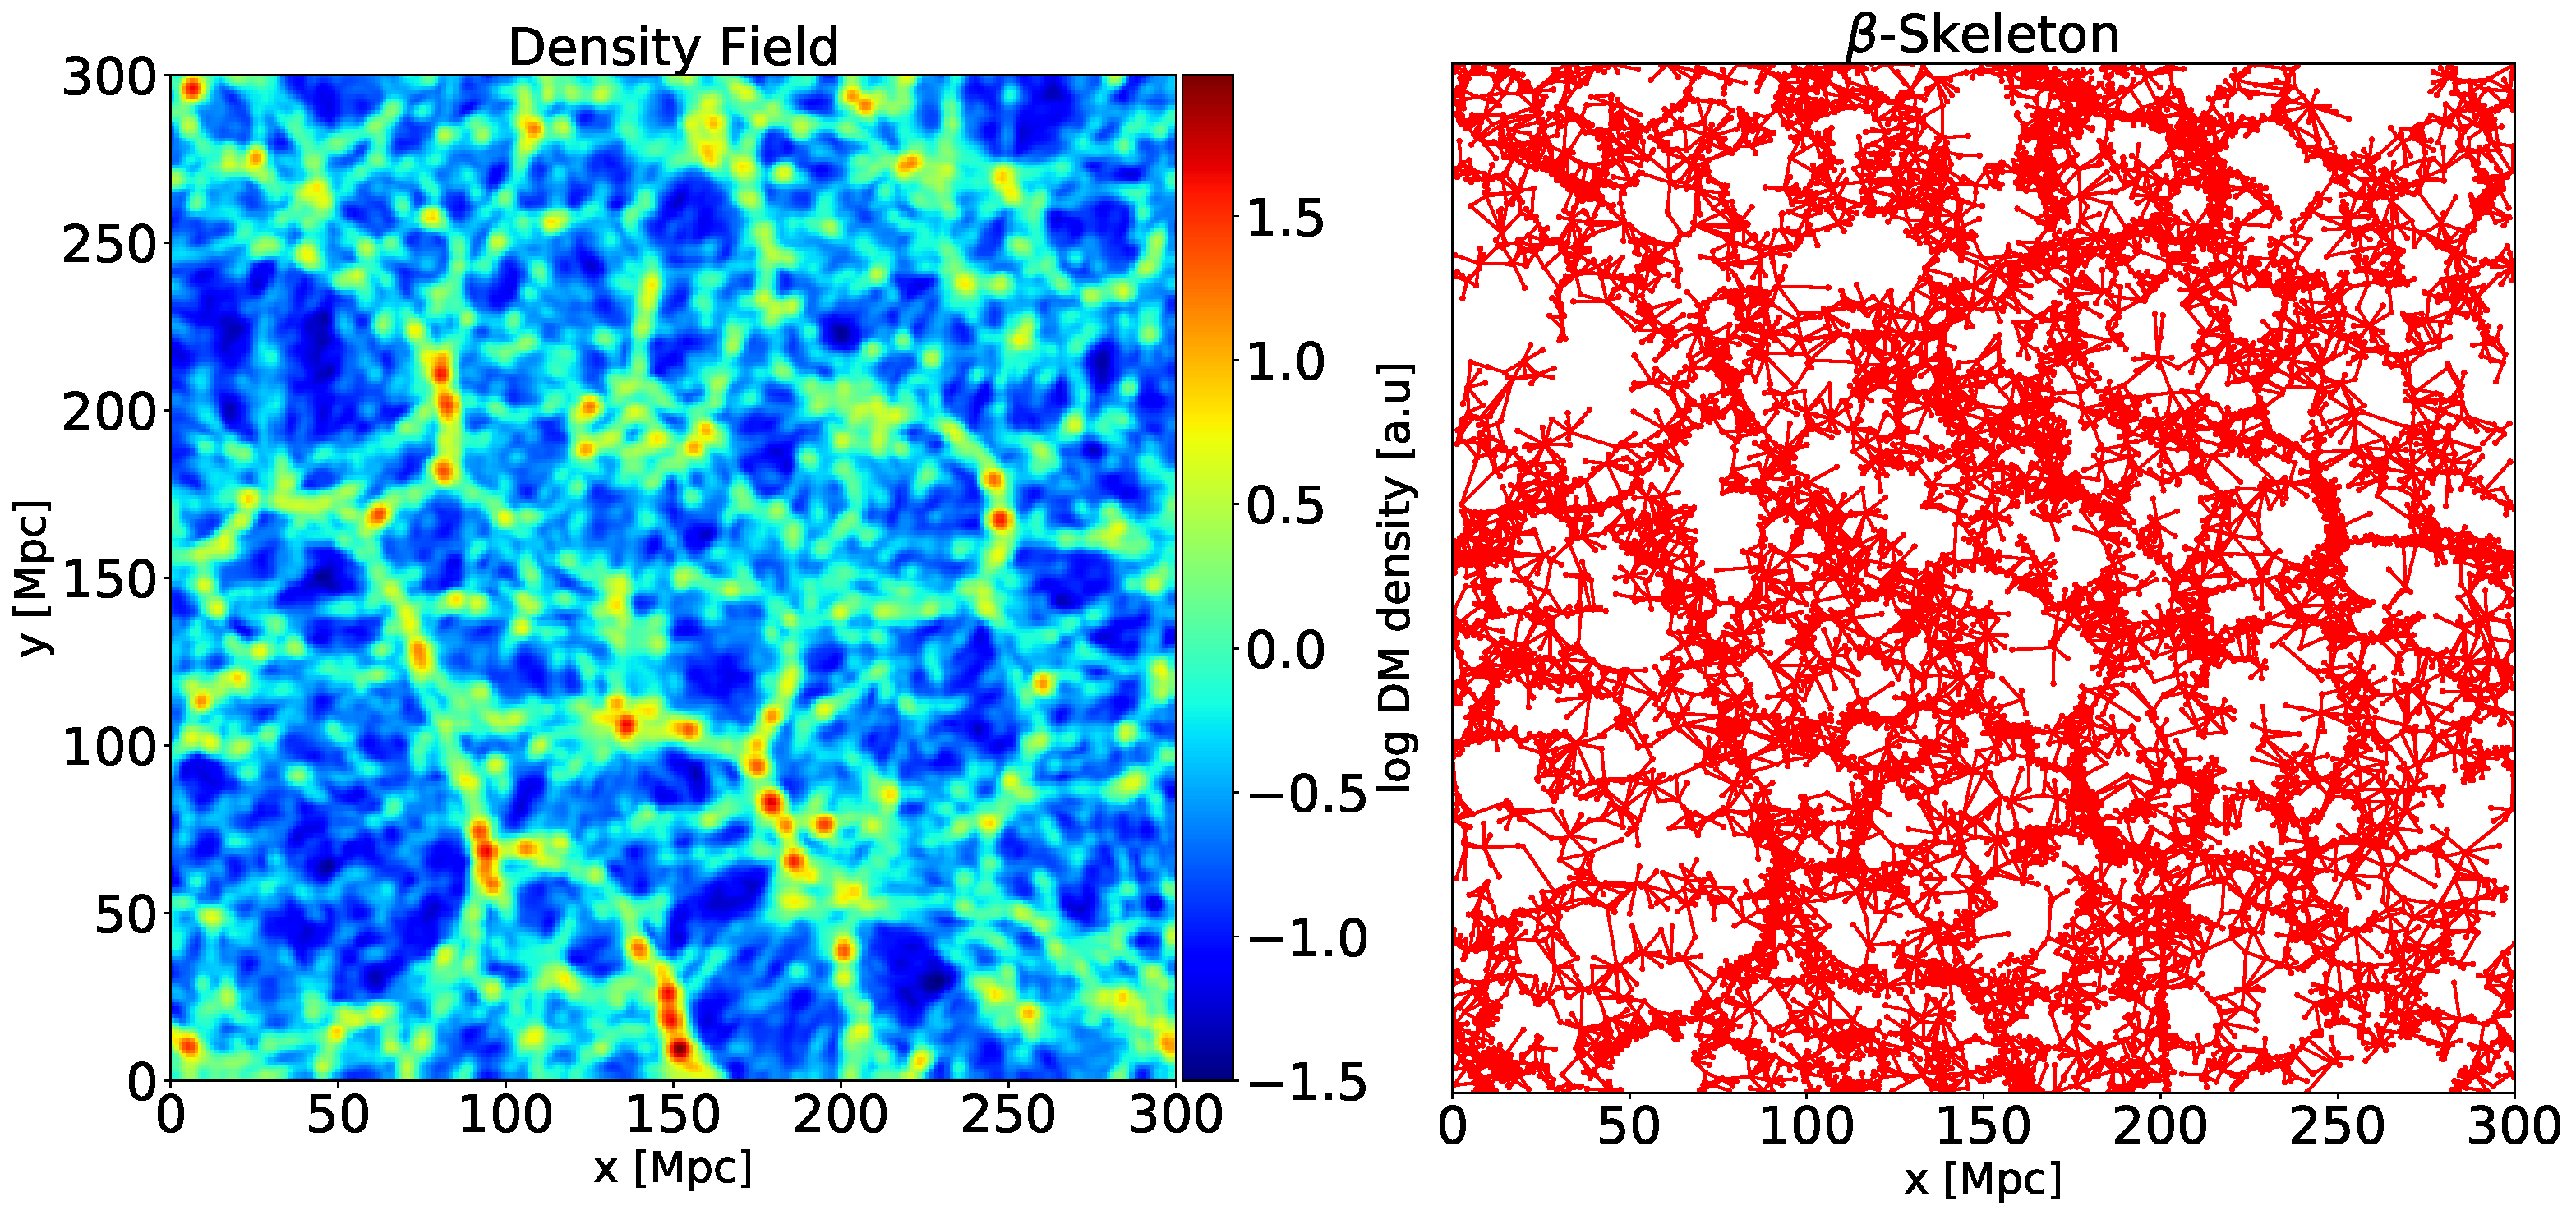
\includegraphics[scale=0.28]{Figs/Fig1_.png}%Figs/p_TWeb_bsk.pdf}
 \caption{Comparison between the T-Web of dark matter density field
   (left) and the $\beta$-skeleton (right) computed from the
   distribution of galaxies with $\beta$=1 for Illustris-TNG300.}  
 \label{fig:TWebBsk}
\end{figure*}


\begin{figure*}
        \includegraphics[scale=0.37]{Figs/p_all_features_correlations.pdf}
    \caption{Histograms and correlations curves for the eight features
      used to train the classifiers.}  
    \label{fig:features}
\end{figure*}

\subsection{The $\beta$-skeleton algorithm}

The $\beta$-skeleton is an algorithm that computes a graph over a
distribution of nodes \citep{Kirkpatrick1985, Fang2019}.  
This algorithm depends on a positive and continuous parameter $\beta$
that defines an exclusion region between two nodes.

{\bf Defining $d$ as the distance between two nodes, they are connected by an edge if any other point is allocated in the various exclusion regions shown in Figure \ref{fig:beta}. 

For $\beta<1$, the exclusion region is the intersection of all the spheres with diameter $d/\beta$ that pass through the nodes. In the case, $\beta=1$, the exclusion region is a sphere with a diameter $d$.  
As $\beta$ increases, $\beta>1$, the exclusion region is larger and it is the intersection of all the spheres with diameter $d\beta$ having the nodes in their boundary.}

This makes that for low values of $\beta$ the graph is dense and for
large values of $\beta$ the graph becomes sparse. 
The $1$-skeleton also receives the name of Gabriel Graph.  
The $2$-skeleton is also known as the Relative Neighbor Graph (RNG).

In our case, the galaxies represent a node in the graph.
From this graph, we compute a variety of features to be used as an
input for the classification task.  



\section{Linking the $\beta$-skeleton to the T-Web}\label{sec:link}

Figure \ref{fig:TWebBsk} shows the correlation between the DM overdensity
and the $\beta$-skeleton graph computed over the corresponding galaxy
distribution. 
This spatial correlation suggests that graph derived features might have
a good chance to predict the DM web environment. 
However, there is a number of free parameters that have to be explored
to find the best match between the $\beta$-skeleton and the cosmic web.

\subsection{T-web and $\beta$-skeleton free parameters}

For a start, the influence of the $\beta$ parameter has to be explored.
Additionally, the classification provided by the T-web algorithm
depends on the smoothing scale, $\sigma$, used to compute the Hessian and the
threshold parameter $\lambda_{th}$ used to define the web elements.
The tracers we use from the simulation can also change. 
We use a simple magnitude cut $M_{r}$ on the $r$-band absolute magnitudes
to define the galaxy sample. 
Different values for that threshold naturally produce different galaxy
distributions and thus different $\beta$-skeletons. 

The T-web computation is performed over a cubic grid with $256^3$
cells.  
This corresponds to a cell size of $1.17$ Mpc.
For the smoothing parameter we take five different values of $\sigma =
0.5$, $1.0$, $1.5$, $2.0$ and $2.5$, expressed in units of the cell
size on a side.   
In turn, for each smoothing length we take five different values for
the eigenvalue threshold
$\lambda_{th}=0.0, 0.1, 0.2, 0.3, 0.4$ and $0.5$. 
We use four different values for the limiting $r$-band magnitude
$M_{r}$ we use  $-18, -16, -14$ and $-12$.
From these galaxies we compute the skeleton using values of $\beta$ in
the range $1\leq \beta \leq 2$ to find that the best results are
obtained for $\beta=1$.   
Therefore we keep this value fixed for the results reported here.

Once these four different parameters ($\beta$,
$\sigma$, $\lambda_{th}$ and $M_{r}$) are fixed the $\beta$-skeleton and the
T-web are fixed.  
Next we define what features used to predict the four cosmic web elements.

\subsection{Galaxy Features}
We use eight features for each galaxy in the $\beta$-skeleton to train the classifiers. 

\begin{enumerate}
\item[1)]
The number of connections minus the global average number of
connections, $\eta = N_c - \bar{N}_c$. 
\item[2)]
The ratio between the average edge length to first neighbors on the graph
normalized by the global average edge length, $\delta=D_{av}/\bar{D}_{av}$. 
\item[3)] 
The logarithm of the pseudo-density over the graph,
  $\varrho=\log_{10}\rho$.   
This pseudo density $\rho$ is defined as the inverse of the volume
computed from the ellipsoid that best fits the distribution of first
neighbors over the graph. 
If a galaxy has less than three neighbors its volume is fixed to be $10^{-4}$.
\end{enumerate}
\noindent
We define three more features that we call $\Delta$-features.
Their values are computed as the difference between the corresponding
value in a node and the average value over first neighbors nodes.  
They can be loosely interpreted as a first derivative computed over the graph. 

\begin{enumerate}
\item[4)] $\Delta$ over the number of connections, $\Delta\eta$.
\item[5)] $\Delta$ over the normalized edge length, $\Delta\delta$.
\item[6)] $\Delta$ over the the pseudo-density, $\Delta\varrho$.
\end{enumerate}

\noindent
Two more features come from the $r$-band magnitudes
\begin{enumerate}
\item[7)] The absolute $r$-band magnitude, $M_r$.
\item[8)] $\Delta$ over the absolute $r$-band magnitude, $\Delta M_r$.
\end{enumerate}

Figure \ref{fig:features} show the correlations among all features.
The diagonal panels present the distribution of a given parameters.
The strongest correlations are present for the the average number of
connections $\eta$, the connection length $\delta$, the
pseudo-density $\varrho$ and the r-band magnitude $M_r$ with their
corresponding $\Delta$ features.





\subsection{Classification Algorithms}

We explore three different supervised machine learning algorithms to
predict the cosmic web environment from the features we have just
presented. 
For each algorithmthe most relevant metaparameters driving their
performance.

\begin{itemize}
    \item Support Vector machines: 
        \begin{itemize}
            \item kernel: Radial basis function
            \item Regularization parameter $C$=0.01, 0.1, 1.0.
            \item Scale for the radial basis function  $\gamma$=0.01, 0.1, 1.0.
        \end{itemize}
        For this algorithm we standardize the input features to have
        mean zero and standard deviation of one. 
    \item Classification trees
      \begin{itemize}
      \item Maximum tree depth: From 1 to 30.
      \end{itemize}
    \item Random forest
        \begin{itemize}
            \item Maximum tree depth: 10.
            \item Number of estimators: From 1 to 100.
        \end{itemize}
\end{itemize}

\subsection{Model evaluation}

After computing the features we discard the galaxies located within 5 Mpc
away from the box limits  in order  to avoid boundary effects coming
from incomplete $\beta$-skeleton information.  
From this set we randomly select $50\%$ of galaxies to train the ML
algorithms.   
We use another $30\%$ as validation to find the best algorithm and ML
meta-parameters together with the best matching T-web and
$\beta$-skeleton parameters.   
Finally, we use the final $20 \%$ of data as test to report
on the expected confusion matrix and feature importance for the
classification. 

As performance metrics we compute the precision, recall and the F1
score (harmonic mean between precision and recall).  
We compute the F1 for each web environment and its average.


\begin{figure}
    \includegraphics[scale=0.55]{Figs/p_hist_f1.pdf}
    \caption{Histograms of the average F1 for the three machine
      learning algorithms.
      The average F1 changes as the parameter and meta-parameter
      are changed.}
    \label{fig:methods}
\end{figure}



\begin{table}
\centering
\begin{tabular}{p{1.8cm}ccc}
\hline
                  & Random               & Classification        & SVM\\
                  & Forest               & Trees                &  \\
\hline
 F1 Peaks               & 0.52 $\pm$ 0.26  & 0.46 $\pm$ 0.24 & 0.42 $\pm$ 0.09  \\
 F1 Filaments          & 0.71 $\pm$ 0.05 & 0.66 $\pm$ 0.07 & 0.33 $\pm$ 0.09 \\
 F1 Sheets             & 0.55 $\pm$ 0.05 & 0.50 $\pm$ 0.10 & 0.26 $\pm$ 0.09 \\
 F1 Voids              & 0.27 $\pm$ 0.18 & 0.27 $\pm$ 0.17 & 0.12 $\pm$ 0.09 \\
 Average F1\\ with voids    & 0.51 $\pm$ 0.08 & 0.47 $\pm$ 0.09 & 0.28 $\pm$ 0.06 \\
 Average F1\\ without voids & 0.59 $\pm$ 0.08 & 0.54 $\pm$ 0.08 & 0.34 $\pm$ 0.07 \\
\hline
\end{tabular}
\caption{Mean values and standard deviations over the F1
  scores for the 20 best models in each one of the ML algorithms.
  The first four rows differentiate the results for each one of the
  environemnts.
  The fifth row corresponds to the unweighted average over the four
  web elements, while the last row is the average over web elements
  with the exclusion of voids.}
\label{table:elements}
\end{table}

\section{Results}\label{sec:results}


\subsection{ML algorithm performance}


We start by comparing the performance of the different ML algorithms.
Figure \ref{fig:methods} shows the average F1 distribution for
all the classification experiments. 
The histograms are discriminated into the three ML algorithms.
The first result that stands out is that SVM shows the worst
classification results.
The F1 score is the average F1 over the four web environments.

The mean values of this average F1 score for SVM is around 0.3, while its best
value is close to 0.5.
For Classification Trees and Random Forest the results are notably better. 
The mean value over the distribution is close to 0.5 while their best
average F1 is close to 0.6.
From these two models, the results from the Random Forest are
better; the F1 value distribution is skewed towards higher values than
the distribution from the Classification Tree.
From this overall response over all possible models, Random Forest
emerges as the best ML algorithm.
We can confirm this result by performing a more detailed analysis by
taking a look at the reults for each cosmic web element separately.


Table \ref{table:elements} summarizes the F1 performance split by cosmic
web element in the first four rows.
The mean values and standard deviations are computed over all the ML
experiments. 
From this table we confirm that the RF classifier performs
consistently better than CT and SVM for every web element.
The F1 scores from RF are always at least 0.15 above SVM.
The comparison between RF and CT shows that for peaks, filaments and
sheets the RF produces average F1 scores 0.05 higher. 
However, for voids the average of the scores are similar. 

\subsection{Performance across web elements}

Table \ref{table:elements} also shows that some cosmic web elements 
are harder to predict than others.
Focusing our attention on the RF classifier, the algorithm with the
best results,  we readily observe that filaments is the environment
with the best mean F1 score (0.71).
This score is followed by sheets and filaments (0.55 and 0.51,
respectively) and finally by voids (0.27). 

Void is the hardest class to predict. 
The reason behind this result is easy to understand. 
There are too few galaxies in voids. 
Across all models, Less than XX $\%$ of all galaxies
are classified as void galaxies. 
This has two consequences.
First, the low number of instances makes it hard for the ML algorithm to
define the region in parameter space occupied by voids.
Second, a small number of void galaxies that are missclassified is
translated into large changes in the F1 scores.


\subsection{Best parameters and metaparameters}


best models from all the three different ML algorithms.
We choose the best $20$ results in terms of the average F1 to understand
in detail the algorithm performance and the influence on the 
different web elements classification.
Considering the best $10$ or $50$ models does not affect the results
and insights we are about to present.




Figure \ref{fig:prediction} shows the comparison between the ground
truth environments (left) and the prediction (right) by the best ML algorithm
with the optimized parameters and meta-parameters  for the best
method. 
The visual impression is that the sheets and filaments have good predictions,
peaks are reasonable, while voids are the worst. 




To evaluate the methods, it was computed the mean values and errors
for the 20 larger F1 score by method. Table \ref{tab:methods} show mean
values for the F1 by environment and the averages considering voids 
and not. 
In general, in both cases, the evaluation shows that the best method is
the Random Forest.  


The Random Forest have other types of configurable parameters, the
most common parameter is the number of estimators NE, we evaluate the
Random Forest with the F1 score as a function of the NE parameter.  
Figs.\ref{fig:F1_curve} show the behavior of the F1 average score as a
function of NE in contrast to the populations of the environments,
the left figure shows the F1 average score,
the maximum is near to 0.6.
The center figure shows the F1 score for the four environments,
the best environment predicted is the filaments followed by the peaks and sheets,
the worst predicted environment is the voids,
this due the population of them as we can see in the right figure of the Fig.\ref{fig:F1_curve},
we can observe that the amount of voids is considerably less than the
others environments almost in one order of magnitude. 

Including the NE meta-parameter, the Fig. \ref{fig:features_void} (upper)
shows the distributions of all meta-parameters for the 20 best results
using Random Forest and the F1 average distribution. We can observe that the meta-parameter $\lambda_{th}$
is 0.5 and $\sigma$ have values of 1.5 and 2. For these
values of $\lambda$ and $\sigma$ the number of galaxies in voids is not real according with our analysis. Due to this inconsistency, we can consider the meta-parameters filtering when the F1 average is computed excluding the voids. The table \ref{tab:metaparameters} show the combinations of meta-parameters that allow us to obtain a good prediction. The distribution of these meta-parameters
in the case when we do not consider the voids in the F1 average score is shown in Figure \ref{fig:features_void}(bottom). We can
observe in this Figure that the threshold $\lambda_{th}$ is 0.1, the smoothing $\sigma$ 1.5 and 2, and the luminosity $M_r$<-14. The NE varies between 23 and 100 but is concentrate in values larger than 80. 

The bad prediction of the voids illustrated in the Figure
\ref{fig:F1_curve} is confirmed by the results shown in
Figure \ref{fig:confusion_matrix}(left) computed for the 20 best models.  

In the Fig. \ref{fig:confusion_matrix}(left) we observe that the best prediction is for filaments where the $80\%$ of the true galaxies in filaments are correctly predicted. 
This fraction is followed by $63\%$ of correct peaks, $55\%$ of
correct sheets galaxies with a low value of $8\%$ void galaxies
classified correctly. 

Fig.~\ref{fig:confusion_matrix}(right) shows the importance of the features
for the 20 best Random Forests models. According to the Figure, the 
most important feature is $\Delta \delta$
related to the local average distance between connections, followed by
the local number of connections $\Delta \eta$. This Figure shows
us that the separation between the galaxies is a parameter that can determinate the T-Web environment for a galaxy. 

We report the best results using the validation data, the
Fig. \ref{fig:confusion_matrix_valid}(left) shows the confusion matrix
for the validation data with the best model where $\lambda_{th}$=0.1,
$\sigma$=1.5, $M_r$=-14 and $NE$=80. The
Fig. \ref{fig:confusion_matrix_valid}(right) shows the feature
importances for the validation data, we can observe that the local
average distance $\Delta \rho$ and the local number of connections
$\Delta \eta$ remain the most important according with the results
obtained for the test data. 

The best model was evaluated including the information of the features
extracted from the 2 and 3-skeleton, the results do not vary in
comparison when we used only the features of the 1-skeleton, these
showed that the 2 and 3-skeleton do not contain important information
to predict the T-Web. 




\begin{figure*}
\centering
    \includegraphics[scale=0.23]{Figs/p_features_Forest_F1_av.pdf}
    \includegraphics[scale=0.23]{Figs/p_features_Forest_F1_av_no_voids.pdf}
    \caption{(Upper) Distribution of the meta-parameters and the F1 average
      when the voids are including in the average. We can observe that
      the $\lambda$ meta-parameter is 0.5, while $\sigma$
      jumps between 1.5 and 2.0, $M_r$ is -16 mainly and $NE$ are concentrate in 100.
      (Bottom) Distributions when the voids are not including in the average. We can observe that
      the $\lambda$ meta-parameter is 0.1, while $\sigma$
      jumps between 1.5 and 2.0, also, $M_r$ is -14 and $NE$ have a peak in 80.
      } 
    \label{fig:features_void}    
\end{figure*}



\begin{table}
\centering
\begin{tabular}{rrrr}
\hline
   $\lambda$ &   $\sigma$ &   $M_r$ &   $NE$ \\
\hline
         0.2 &        1.5 &     -14 &     67 \\
         0.2 &        1.5 &     -14 &     78 \\
         0.1 &        2   &     -14 &     89 \\
         0.1 &        2   &     -14 &     78 \\
         0.1 &        2   &     -14 &    100 \\
         0.1 &        2   &     -16 &     34 \\
         0.1 &        2   &     -16 &     45 \\
         0.1 &        1.5 &     -14 &     34 \\
         0.1 &        1.5 &     -14 &     67 \\
         0.1 &        1.5 &     -14 &     56 \\
         0.1 &        1.5 &     -14 &     45 \\
         0.1 &        1.5 &     -14 &     23 \\
         0.1 &        2   &     -16 &     56 \\
         0.1 &        1.5 &     -14 &    100 \\
         0.1 &        1.5 &     -14 &     78 \\
         0.1 &        1.5 &     -14 &     89 \\
         0.1 &        2   &     -16 &     67 \\
         0.1 &        2   &     -16 &    100 \\
         0.1 &        2   &     -16 &     78 \\
         0.1 &        2   &     -16 &     89 \\
\hline
\end{tabular}
\caption{Values of the meta parameters for the best 20 models using Random Forest with the test data when we do not consider the voids in the F1 average score.}
\label{tab:metaparameters}
\end{table}


\begin{figure*}
\centering
    \includegraphics[scale=0.32]{Figs/p_confusion_matrix_valid.pdf}
    \includegraphics[scale=0.28]{Figs/p_features_importance_valid.pdf}  
    \caption{(Left) Confusion Matrix (CM) for the valid data with the
      best model $\lambda_{th}$=0.1, $\sigma$=1.5, $M_r$=-14 and
      $NE$=80. The best prediction are obtained for the 
      filaments, where the $81\%$ was predicted correctly. The worst
      prediction was for the voids where only the $6\%$ was predicted 
      correctly.
      (Right) Feature importance for the valid data. The most
      important feature is the local average distance $\Delta\delta$
      with a $32\%$ of importance, follow by the local number of
      connections with a $27\%$ of importance.}  
    \label{fig:confusion_matrix_valid}
\end{figure*}

\begin{figure*}
  \centering 
    \includegraphics[scale=0.25]{Figs/p_environment_predicted.pdf}
    \caption{Comparison between the DM T-Web from the Illustris-TNG
      simulation and the environments predicted by the Tree Classifier
      algorithm.} 
    \label{fig:prediction}
\end{figure*}


\section{Conclusions}\label{sec:conclusions}

In this paper we presented a method to predict the dark matter cosmic web
environment of a galaxy from its neighbor graph information.
We used the T-web as the cosmic web definition \citep{Forero-Romero2009}
and the $\beta$-skeleton graph \citep{Fang2019} 
to describe the relative spatial distribution of the galaxies. 
The link between the T-web and the graph is done through different
machine learning algorithms: support vector machines, random forests and
classification trees.

We test the method using data from the Illustris-TNG simulation.
The T-web is calculated on a grid of cell size $0.8$\Mpch 
and a Gaussian smoothing scale $\sigma$ and an eigenvalue threshold $\lambda_{th}$.
The $\beta$-skeleton is computed over galaxies brighter than 
an $r$-band absolute magnitude cut $M_{r}$.
For each simulated galaxy we build the $\beta$-skeleton and
compute features such as the number of connections, the average connection
length, the pseudo-density and the difference of these quantities with
respect to the average over first-neighbors.

We find that the T-web environment that is best predicted has smoothing
scale of $\approx1.5$ \Mpch and an threshold $\lambda_{th}=0.1$. 
This turns out to be the ballpark range favored in previous publications
for T-web  studies for the resulting classification to match the visual impression of the cosmic web \citep{Forero-Romero2009}.
We also find that the features computed with the $1$-skeleton 
(Gabriel Graph) are enough to obtain good predictions. 
The best classification results are not sensitive to the $r$-band
magnitude cut, although a cut of $M_r>-14$ gives the best results.

The best algorithm to predict the environment are the random forest followed closely by classification trees. 
Support Vector Machines provide the worst results.
From the random forest we are able to determine that the two most
important features for the environment classification are the average connection length and number of connections over the neighbors with respect to the average over its first neighbors.

The environments that are best predicted are in decreasing order: 
filaments, peaks, sheets and voids. 
This ranking follows the number of galaxies found in each of these environments.
Galaxies in voids represent less that $2\%$ of the total number of galaxies and 
are the hardest class to predict, with $F1$-scores of $\approx0.6$.
Motivated by this limitation, in future work we will present a method to define
voids from the $\beta$-skeleton graph.

All the results we reported here were obtained using a single snapshot at a 
redshift $z=0$.
Our results provide the baseline for future work that will have to quantify 
the effect of redshift space distortions and survey incompleteness in order to
predict  the DM T-Web form survey data.
Nevertheless, the two most interesting features of our method are: a) it does not
rely either on binning the galaxy data on a grid and b) it does not require a dark matter density reconstruction.



\section*{Acknowledgements}

We are thankful to the community developing and maintaining open source packages fundamental to our work: numpy
\&  scipy  (Walt  et  al.  2011),  the  Jupyter  notebook  (P\'erez \& Granger 2007; Kluyver et al. 2016), matplotlib (Hunter2007) and  scikit-learn (Pedregosa et al. 2011).
%%%%%%%%%%%%%%%%%%%%%%%%%%%%%%%%%%%%%%%%%%%%%%%%%%

%%%%%%%%%%%%%%%%%%%% REFERENCES %%%%%%%%%%%%%%%%%%
% The best way to enter references is to use BibTeX:
\bibliographystyle{mnras}
\bibliography{references}

% Alternatively you could enter them by hand, like this:
% This method is tedious and prone to error if you have lots of references
%\begin{thebibliography}{99}
%\end{thebibliography}
%%%%%%%%%%%%%%%%%%%%%%%%%%%%%%%%%%%%%%%%%%%%%%%%%%

%%%%%%%%%%%%%%%%% APPENDICES %%%%%%%%%%%%%%%%%%%%%
%\appendix
%\section{Some extra material}
%%%%%%%%%%%%%%%%%%%%%%%%%%%%%%%%%%%%%%%%%%%%%%%%%%

% Don't change these lines
\bsp	% typesetting comment
\label{lastpage}
\end{document}
% End of mnras_template.tex
